\chapter{Feed 流优化工作}

\section{预渲染框架的背景}

在视频 Feed 流中,对于下一个视频信息的加载逻辑处理通常是需要格外小心的。因为该过程发生在用户滑动屏幕的时候,此时主线程正不断接收用户发送的滑动事件,并根据这些滑动的事件来进行布局、UI 刷新等操作,占据了主线程很大一部分资源。如果这个时候数据绑定的流程过于复杂,会严重增加这段时间的主线程耗时,从而影响整体的流畅性,甚至造成肉眼可见的卡顿。因此,在 Adapter 进行数据绑定的过程中,是强烈不建议在主线程进行任何耗时任务的。这些任务要么通过异步的方式后续补齐,要么针对具体的业务,寻找合适的时机提前进行。

然而,经过业务的不断迭代,数据绑定的耗时一定会随着业务方不断添加新的功能而增加。因此,我们希望能够对这个过程进行彻底的优化。在视频 Feed 流滑动的过程中,通常用户最希望看到的是下一个视频的封面立刻展示在屏幕上。为了达到这样的目标,通用的方案有针对图片、视频参数等数据做异步加载,同时在播放器的方面也进行一定程度的预渲染。但是由于 RecyclerView 整体的刷新流程是固定的,所以数据绑定是一个必要的过程。不过在对 RecyclerView 进行了足够多的调研之后,我们可以着手进行更加深度的优化,也就是能够在一个合适的时机将整个数据绑定操作提前进行,而不是只异步化其中的一小部分。在视频 Feed 流的场景中,合适的时机是比较容易寻找的,因为用户在滑动到一个视频之后通常会停留一段时间进行交互行为。但是这样的优化会让 RecyclerView 的生命周期产生混乱,因此即使能够做到,也需要经过细致的修复来让其能够准确地派发原先的生命周期。

\section{问题分析和技术选型}

想要优化从滑动屏幕到用户感知卡片刷新的时间,我们不能仅仅通过正面优化绑定的行为来缩短耗时。事实上,业界内已经有一些在合适的时机进行预渲染的手段,同时也不会影响原来的生命周期分发。然而基于 RecyclerView 的 Feed 流并没有提供这样的能力。根本原因是 RecyclerView 更多还是用于处理非粘性滑动的大量图文类型的 Feed 流。因此,我们希望能够给已经在业务方面严重耦合了 RecyclerView 的 Feed 流提供预渲染的能力,提高流畅性体验。

经过调研,目前在 Android 移动端能够实现预渲染的手段主要有以下几种:

\begin{enumerate}
    \item 使用 ViewPager2 来实现预渲染,并且能够简单的封装得到完整的生命周期分发;
    \item 将 RecyclerView 的高度修改为原屏幕高度的2倍,让不可见的那部分承载预加载的 View;
    \item 通过 LayoutManager 设置额外的布局空间,从而在布局过程中多布局一部分。
\end{enumerate}

下面针对当前 Feed 流的业务场景,分析这些优化手段。首先,如果通过重构为 ViewPager2 来实现预渲染,会损失很多 RecyclerView 的灵活性,同时由于在优化项目启动时往往业务逻辑已经非常繁重,所以不可能在短时间内进行大规模的重构;而如果选择将屏幕高度修改为原来的2倍,缺点也非常明显。原本 RecyclerView 在滑动的过程中只需要维护当前 View 和新滑入的 View,在静止时只需要维护正在播放的 View;然而在修改之后需要维护的 View 个数会成倍增加,导致业务逻辑更加繁重,并且其它业务方(如播放器,交互,弹幕,推荐系统等)都需要做不同程度的适配。这样做的工作量也是非常大的。

因此,最终我们选择第3种方案,也就是通过 LayoutManager 提供的额外布局能力来实现预渲染。这样对 RecyclerView 本身的改动非常小,同时也只是将数据绑定的时机提前。不过,这样的改动依然会对业务造成不小的影响,所以需要对改动带来的副作用进行全方位的排查并在框架层面进行适配。

\section{预渲染框架的设计思路}

预渲染框架整体分为两部分:经过修改的 PreloadLinearLayoutManager 和派发卡片可见性事件的 ViewHolderVisibilityDispatcher。前者主要是替代原有的 LinearLayoutManager,用于实现多种模式的预渲染。同时也对一些由于预加载导致的异常情况进行了修正;后者是由于原来的数据绑定无法再被用于确定卡片是否对用户可见,从而引入的新的生命周期分发器。业务方可以注册卡片的可见性监听器,并将原来依赖于数据绑定的行为(如曝光埋点)迁移至新监听器的回调方法中。下面对于两个组件的具体实现以及设计架构进行说明。

\subsection{实现预渲染逻辑}

LinearLayoutManager 允许提供额外的布局空间,来处理布局过程中对超出屏幕的部分进行布局的特殊要求。方式是通过重写 getExtraLayoutSpace() 方法或者 calculateExtraLayoutSpace() 方法。其中前者只能向一个方向进行布局,后者可以在两个方向进行布局。但是,如果采用后者的话,没有引入 AndroidX 1.1.0 的项目无法使用。所以使用兼容性更强的 getExtraLayoutSpace()。

在该方法中,可以返回一个整型变量来标识需要额外布局多长的布局空间。因为我们需要额外布局一张卡片(也就是下一个视频的信息),所以返回的距离应该为一张卡片的高度。通常情况下,卡片的宽高信息可以直接通过 LayoutManager 获取到,高度通常为屏幕的高度。

通过这个简单的操作,就已经能够实现预渲染的核心逻辑,并且经过验证已经可以提前绑定下一张卡片的数据。然而,通过验证目前的生命周期,我们可以发现,这样的行为其实和没有预渲染并没有什么不同。我们通过一个例子来进行说明:当前卡片为卡片1,在这个情况下,卡片2会因为额外布局空间也被绑定并创建 View 的实例。这样确实能够达到预渲染的效果;然而,如果用户开始向下滑动,在滑动的一瞬间就会因为额外布局空间,将卡片3也提前创建并绑定。在这种情况下,依然会在滚动的过程中进行数据绑定,只不过从原来的提前一张卡片变成了提前两张卡片,耗时逻辑依然会影响主线程的性能。所以,我们需要对额外布局空间进行限制,只有在应用程序相对空闲的时刻才允许额外的布局空间。反映到业务方就是,选择一个更好的时机去进行预渲染。

为此,设计了若干种预渲染模式,来应对不同业务的需求。主要分为:

\begin{itemize}
    \item 没有预渲染(默认情况);
    \item 永远预渲染;
    \item 滚动停止时触发预渲染;
    \item 通过外界触发预渲染。
\end{itemize}

其中,通过外界触发预渲染的模式还可以分为有超时补发机制和没有超时补发机制。在有超时补发机制的版本中,当滚动停止时,如果外界没有立刻进行预渲染调用,那么就会提交一个默认为5秒的任务。当到达规定时间时如果外界依然没有触发预渲染,那么就会补发一次预渲染来应对异常情况。想要让 LayoutManager 在这些不同的预渲染模式中自如切换是需要经过缜密的设计和严谨的测试的,接下来介绍为了迎合不同的模式进行的工作。

RecyclerView 会分发滚动状态的变化。RecyclerView 的滚动状态一共有三种:

\begin{itemize}
    \item SCROLL\_STATE\_IDLE:静止状态;
    \item SCROLL\_STATE\_DRAGGING:滚动状态,不过是用户将手放在屏幕上时;
    \item SCROLL\_STATE\_SETTLING:滚动状态,用户松手后,还会滑动一段距离直到停止。这段过程的状态就是 SETTLING。
\end{itemize}

当 RecyclerView 处理用户的触摸事件时,会根据具体情况设置滚动状态的标记位,并通过回调方法派发滚动状态改变的生命周期。因此我们可以在回调中监听到新的滚动状态,并针对具体的预渲染模式进行预渲染的派发。当预渲染模式为滚动停止触发预渲染时,如果检测到已经滚动停止,那么应该移除已经存在的预渲染任务,并手动提交一次新的预渲染任务;当预渲染模式为带有超时补发机制的外界触发预渲染时,如果检测到滚动停止,那么会在规定的超时时间后手动提交一次新的预渲染任务。

加入了这些回调逻辑之后,需要对 LayoutManager 的 getExtraLayoutSpace() 做进一步特殊处理。由于我们不会永远预渲染,返回的额外布局空间就不会是一个定值。我们需要针对不同的预渲染模式,根据具体的情况进行判断。如果是滚动停止触发预渲染的模式,只有在当前 RecyclerView 不为滚动状态时才返回额外的布局空间,否则返回默认值0;如果是外界触发的预渲染,那么绝大多数情况都应该返回默认值,只有外界触发预渲染的那一刻才返回额外的布局空间用于预渲染。

以上的逻辑可以满足大部分预渲染的场景。但是,由于没有经过完善的测试,这样的逻辑依然隐藏了一些缺陷。这里主要介绍一下针对预渲染框架进行的额外工作;在下一节会介绍测试环节中出现的缺陷及其解决思路和过程。

主要的额外工作都在外界触发预渲染上,因为外界触发预渲染的时机不能保证。准确地说,无法确保外界触发预渲染时,RecyclerView 一定处于滚动停止状态。因此需要引入不同于超时补发预渲染机制的另一种补发预渲染的时机:当外界触发预渲染时,如果 RecyclerView 还不处于滚动停止状态,那么需要等到滚动停止时进行补发。这样做的一个主要原因是,在视频场景的 Feed 流中,通常外界触发预渲染的时机是视频起播的时机。但是视频起播通常和滚动停止互为异步行为。这样做的目的是为了优化起播的速度,用户滑动到当前视频,在卡片停稳之前就能做一些初始化的工作,从而让用户感觉视频的播放更加流畅。而如果视频起播时卡片仍然在滑动(性能越强的手机越容易出现这种情况),那么就违背了让预渲染任务避开卡片滑动事件的初心。因此需要做这样一个补发机制,来让外界触发的预渲染一定是在卡片静止时进行的。为此设置了如下标记位来记录外界触发预渲染模式下的特殊状态:

\begin{itemize}
    \item 是否给予短暂的额外布局空间:这个标记位只有预渲染任务触发时才设置为真。当用户再次滑动后,需要设置为假,以保证外界触发的预渲染只会执行一次;
    \item 超时时间:当预渲染模式为带有超时补发机制的外界触发预渲染时,记录超时的时间。在这个时间之后,提交的预渲染任务会被执行。如果在超时时间之内已经有预渲染任务被执行,该任务会被取消;
    \item 不幸的外界尝试:当外界触发预渲染时,如果卡片仍处于滚动状态,会被设置为真。在下一次(通常是很短的时间之后)RecyclerView 滚动停止时,会针对这个不幸的尝试进行补发,并再次将标记位设置为假。
\end{itemize}

当 getExtraLayoutSpace() 被执行时,如果当前处于外界触发预渲染的模式,就会根据这些标记位来决定是否分发额外的布局空间。

下面介绍对于不同的预渲染模式下,PreloadLinearLayoutManager 与 RecyclerView 配合在滑动屏幕时进行布局的具体行为。

传统的 RecyclerView 在滑动中的布局行为见图 3.1:当滑动产生时,RecyclerView 会拦截 ACTION\_MOVE 事件,在 onTouchEvent() 方法中处理滑动事件,并在此处真正触发滚动流程。滚动的过程本身就是在不断消费滚动事件,对于每一个滚动的事件,需要判断滚动的方向,并沿着这个方向给出最终滚动的距离,最后用这个距离去进行布局,在布局的过程中同步处理 View 的回收和复用。在计算距离的过程中,还会考虑到是否有额外的布局空间。如果有的话,会额外进行一段布局。

\begin{figure}
    \centering
    \begin{adjustbox}{max width=\textwidth}
        \begin{tikzpicture}[node distance=3cm,>=latex']

            % Define block styles
            \tikzstyle{decision} = [diamond, draw, fill=blue!0, 
                text width=4.5em, text badly centered, inner sep=0pt]
            \tikzstyle{block} = [rectangle, draw, fill=blue!0, 
                text width=5em, text centered, rounded corners, minimum height=3em]
            \tikzstyle{line} = [draw, -latex']
            
            % Nodes
            \node [block, text width=8em] (touch) {手指开始滑动};
            \node [block, right of=touch, text width=10em, node distance=8cm] (scroll) {RecyclerView 接收到滑动事件};
            \node [block, below of=scroll, text width=10em, node distance=6cm] (start_scroll) {RecyclerView 开始布局流程};
            \node [decision, left of=start_scroll, node distance=7cm] (extra) {是否需要额外布局空间};
            \node [block, below of=extra, node distance=4cm, text width=20em] (extral_ayout) {进行布局,在布局过程中额外布局一段空间};
            \node [block, above of=extra, node distance=4cm, text width=10em] (normal_layout) {进行普通布局流程};
            % \node [decision, below of=start] (decision) {Decision};
            % \node [block, below of=decision, node distance=3cm] (yes) {Yes};
            % \node [block, right of=decision, node distance=4cm] (no) {No};
            % \node [block, below of=yes, node distance=3cm] (end) {End};
            
            % Paths
            \path [line] (touch) -- (scroll);
            \path [line] (scroll) -- (start_scroll);
            \path [line] (start_scroll) -- (extra);
            \path [line] (extra) -- node[left] {Yes} (extral_ayout);
            \path [line] (extra) -- node[left] {No} (normal_layout);
            % \path [line] (start) -- (decision);
            % \path [line] (decision) -- node[left] {Yes}(yes);
            % \path [line] (decision) -- node[above] {No} (no);
            % \path [line] (yes) -- (end);
            % \path [line] (no) |- (end);
            
        \end{tikzpicture}
    \end{adjustbox}
    \caption{RecyclerView 在滑动中的布局行为}
\end{figure}

在一直预渲染的模式下,流程和图 3.1 一致,只不过判断额外空间时,永远走的是 Yes 分支。

在滚动停止触发预渲染的模式下,相当于替换了额外布局空间的判断流程。只有监听到 RecyclerView 处于静止状态时,才会允许提供额外布局空间,反之则不会允许。不过,由于在此基础上会修复一个缺陷,判断条件会增加一条。详细的条件将在下一章介绍。

外界触发预渲染模式是最复杂的一个模式,同时还具有超时机制,具体的流程如图 3.2。和 RecyclerView 本身处理滑动的流程不同,该流程是在原来布局流程的基础上额外增加的新流程。因为外界触发的预渲染不会有一个确定的触发时机,所以实际上它和滚动过程中的布局互为异步行为。当外界触发预渲染时,如果此时 RecyclerView 不处于滑动状态,可以直接进行额外布局;而如果此时正在滚动,则此时的预渲染应该在滚动停止时补发。所以设置了 unlucky 标记位来记忆补发预渲染;当开始滑动时,在监听新的滚动状态的回调方法中进行如下任务:

\begin{center}
\begin{adjustbox}{max width=\textwidth}
\begin{tikzpicture}[node distance=3cm,>=latex',every node/.style={font=\small}]

    % Define block styles
    \tikzstyle{decision} = [diamond, draw, fill=blue!0, 
        text width=4.5em, text badly centered, inner sep=0pt]
    \tikzstyle{block} = [rectangle, draw, fill=blue!0, 
        text width=5em, text centered, rounded corners, minimum height=3em, minimum width=1em]
    \tikzstyle{line} = [draw, -latex']
    
    % Nodes
    \node [block, text width=8em] (touch) {手指开始滑动};
    \node [block, below of=touch, text width=8em] (receive_scroll) {RecyclerView 接收到滑动事件};
    \node [decision, below of=receive_scroll, node distance=3cm] (is_scroll_touch) {此时是否是滑动状态};
    \node [decision, below of=is_scroll_touch, node distance=4cm] (is_unlucky) {之前是否有不幸的外界预渲染};
    \node [block, right of=is_unlucky, node distance=4cm] (set_unlucky_false) {设置 unlucky 标记位为 false};
    \node [decision, right of=receive_scroll, node distance=4cm] (with_timeout) {是否设置了超时补发};
    \node [block, below of=with_timeout, text width=8em, node distance=3cm] (post_extra_layout) {提交超时任务};
    \node [block, right of=set_unlucky_false, text width=8em, node distance=4cm] (extra_layout) {进行额外布局};
    \node [decision, above of=extra_layout, node distance=4cm] (is_scroll_outside) {此时是否是滑动状态};
    \node [block, above of=is_scroll_outside, text width=8em, node distance=6cm] (outside) {外界触发预渲染};
    \node [block, right of=is_scroll_outside, node distance=4cm] (set_unlucky_true) {设置 unlucky 标记位为 true};
    
    % Paths
    \path [line] (touch) -- (receive_scroll);
    \path [line] (receive_scroll) -- (is_scroll_touch);
    \path [line] (is_scroll_touch) -- node[left] {No} (is_unlucky);
    \path [line] (is_unlucky) -- node[above] {Yes} (set_unlucky_false);
    \path [line] (set_unlucky_false) -- (extra_layout);
    \path [line] (receive_scroll) -- (with_timeout);
    \path [line] (with_timeout) -- node[right] {Yes} (post_extra_layout);
    \path [line] (post_extra_layout) -- (extra_layout);
    \path [line] (outside) -- (is_scroll_outside);
    \path [line] (is_scroll_outside) -- node[right] {No} (extra_layout);
    \path [line] (is_scroll_outside) -- node[above] {Yes} (set_unlucky_true);
    
\end{tikzpicture}
\end{adjustbox}
\end{center}

\begin{itemize}
    \item 首先判断此时是否是滚动状态。如果不是的话,可以查询之前设置的unlucky 标记位。如果为 true,表示之前有一个不幸的外界预渲染等待补发。因此在这里直接进行预渲染;
    \item 然后查询是否设置了超时补发机制。如果外界设置了超时的时间,则提交一个在规定时间后执行的预渲染任务用来兜底。
\end{itemize}

以上流程只是为了控制最终在布局的时候额外空间的大小。在进行额外布局之前,会通过之前提到的“是否给予短暂的额外布局空间”标记位来进行判断。因此在这个流程中也涉及到对额外布局空间的控制;另外,在进行单次外界预渲染时,需要取消掉之前提交的预渲染任务,来避免重复进行预渲染。

% 每一种模式 + 流程图

\subsection{实现卡片可见性分发}

当引入了预渲染机制后,原本的数据绑定生命周期会根据预渲染的模式而被选择性提前执行。这会导致原本依赖于数据绑定即卡片可见的业务逻辑失效。这样的业务通常有曝光埋点、动画的起播逻辑、播放器的监听业务等。这些逻辑如果仍然依赖于现在的数据绑定事件,会意外地在屏幕外被触发,从而再次带来性能上的损失,UI 显示错误甚至数据错误和崩溃。因此,需要引入一个新的生命周期来标识卡片的出现和消失,让依赖于这些时机的业务逻辑进行迁移。

卡片可见性的分发主要依赖于对目标卡片可见性的计算。如果计算出的卡片可见性和上次不同,则分发新的状态。这也就要求我们需要对每次计算出的卡片可见性进行记忆;另一个问题是,我们需要找到所有卡片可见性可能改变的时机,并在这个时机去触发相应卡片的可见性计算。

经过研究给出如下的解决方案:卡片的可见性记忆采用 View 的 tag。因为对 ViewHolder 进行再次封装会增加业务方适配的难度,所以这里进行最小程度的改造。给 View 增加一个新的 tag,来标记该 View 上一次计算得到的可见性。如果发现新的可见性和上一次不同,则分发新的可见性并进行更新;卡片可见性的触发时机如下:

\begin{enumerate}
    \item 滚动触发时:因为会有新的 View 由于滚动而出现,已经存在的 View 因为滚动而消失;
    \item 当 View 由于自动回收、业务逻辑等原因被移除时:此时该 View 的可见性一定为false,无需进行计算;
    \item 当 RecyclerView 的布局流程完成时:针对通过 Adapter 的通知而导致的视图变动进行新的可见性计算。
\end{enumerate}

卡片可见性的计算的具体的逻辑为计算其在布局方向上是否已经离开屏幕。由于全屏视频场景中同时存在的卡片最多有两个,所以不会出现很大的性能损耗。

%% 分发的图。用新的 newComposition.

% \fbox{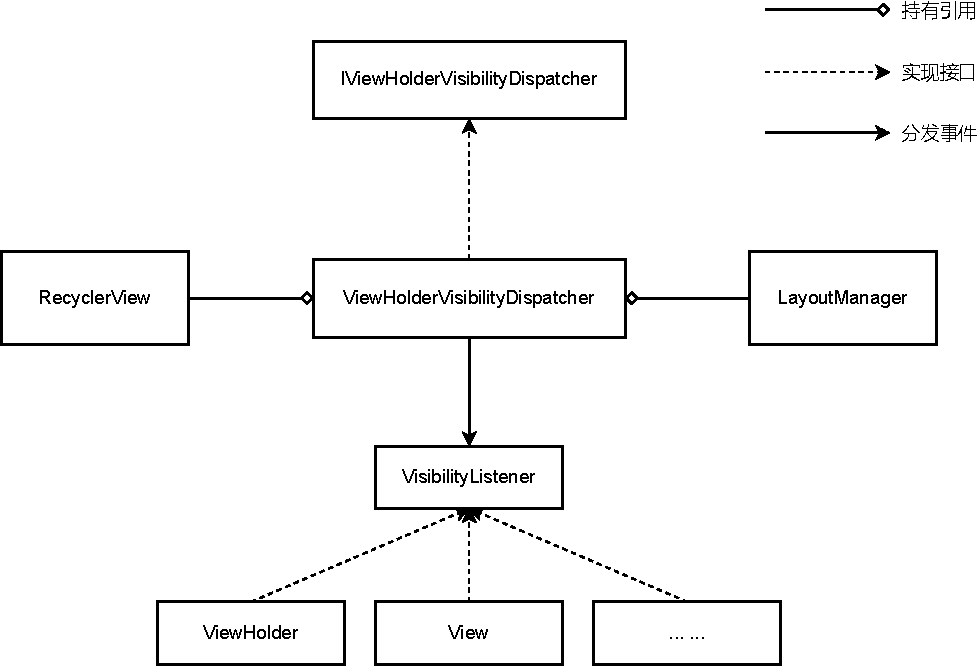
\includegraphics{assets/visibility-dispatch-framework.svg}}

\begin{figure}
    \centering
    \begin{adjustbox}{max width=\textwidth}
        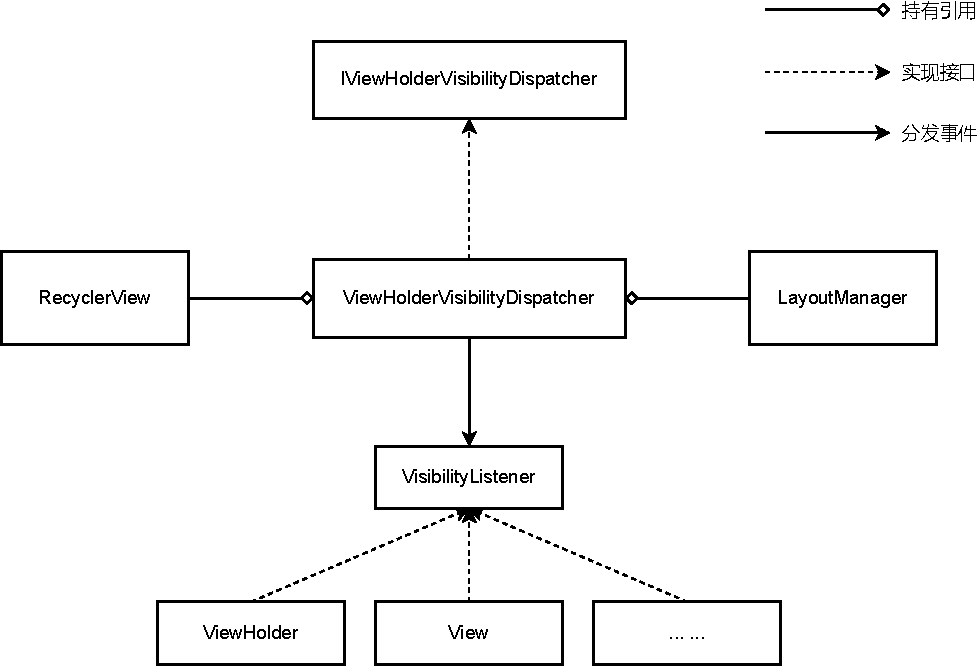
\includegraphics{assets/visibility-dispatch-framework.pdf}
    \end{adjustbox}
    \caption{可见性分发框架设计}
\end{figure}

% 可见性框架的细节

卡片可见性分发的框架设计如图 3.3。ViewHolderVisibilityDispatcher 是主要的卡片可见性事件分发组件,负责核心的可见性计算逻辑以及可见性的记忆和读取操作。由于 RecyclerView 和 LayoutManager 通常在业务中同时初始化,所以将绑定的逻辑也交给 ViewHolderVisibilityDispatcher,让其持有 RecyclerView 和 LayoutManager 的引用,来进行可见性的计算和分发。在相应的时机下,Dispatcher 会将对应的事件分发给 Listener,也就是卡片本身以及监听了可见性事件的业务方组件。在这样的设计模式下,业务方只需要将原来依赖于数据绑定的业务逻辑迁移到新的卡片可见性回调(也就是 VisibilityListener 中的方法)中即可。

\section{预渲染框架的缺陷及其修复过程}

在进行预渲染的测试时,发现了一个对性能影响很大,并且很容易触发的缺陷。如果 RecyclerView 的子 View 处理的触摸事件,并且此时有一个依赖于重置布局的动画在不断播放,那么已经被预渲染的卡片就会在滑动屏幕的一瞬间被回收,随后重新绑定。这样的动画在视频 Feed 流中非常常见。如点赞、收藏等互动的动效,一些广告的贴图,一些吸引用户点击的带有动效的按钮等等。由于我们无法规定业务方是否以重置布局的方式编写,所以我们只能默认这种情况很常见。其实不只是动画,任何重置布局的行为在滑动的一瞬间触发,都有可能导致已经被预渲染出的卡片被回收。所以该缺陷产生的原因必须排查清楚,同时需要在改动尽可能小的情况下尝试修复。

卡片被回收的本质,从预渲染的框架设计中就能看出,一定是因为 getExtraLayoutSpace() 返回了默认值0,并且还是要在卡片没有滚动的状态下。只有上述条件全部被满足,RecyclerView 在布局的时候才会因为没有布局到先前预渲染出的卡片,从而将其回收。然而,用户在这个过程中已经传递了 ACTION\_MOVE 事件,意味着滚动行为已经开始。在这个过程中的布局流程,是一定能够布局到预渲染出的卡片的。这代表很可能有其它布局流程在这个过程中被插入到了滚动流程之前,同时 RecyclerView 此时也已经处于滚动状态。顺着这个思路排查,最终注意到了刚才提到的动画。在真实的业务场景中,屏幕上的很多动画都是通过触发布局流程实现的。改变 View 本身的参数,随后调用 requestLayout() 在下一帧中触发布局流程,从而实现动画的效果。这样的动画虽然会影响性能,但是实现简单,同时如果是简单的动效,对于大盘性能的影响不大。所以在大型项目中这样的动画很常见,并且发生的频率也很高。

根据上述发现,怀疑是业务场景中出现的动画影响了 RecyclerView 布局流程,从而导致卡片误回收。然而,在我自己开发的测试项目中进行复现,并没有出现卡片被回收的情况。所以进一步进行调研 RecyclerView 拦截滑动事件、处理滑动事件并设置滚动状态和开始滚动的全链路,找到其中隐藏的问题。

任何 View 处理滑动流程时,都需要处理 ACTION\_DOWN 事件、ACTION\_MOVE 事件和 ACTION\_UP 事件。通常,一个完整的滑动流程是一个 ACTION\_DOWN 加上若干个 ACTION\_MOVE 以及结尾的 ACTION\_UP。因此,对于 RecyclerView 来说,如何处理 ACTION\_DOWN 事件的走向尤为重要,这影响了后续事件的分发,自然也影响了整个的滑动流程。当 ACTION\_DOWN 事件产生时,RecyclerView 并不会拦截该事件,只会将事件传递给子 View。而子 View 可以自主选择是否消费该事件。如果子 View 没有消费 ACTION\_DOWN,那么将会由 RecyclerView 自己来消费。RecyclerView 本身永远会消费任何触摸事件,所以无法再继续向上传递。之后所有的 ACTION\_MOVE 事件以及最后的 ACTION\_UP 事件都会由 RecyclerView 自己来消费。这也是滑动流程中最理想的情况,完全由 RecyclerView 来主动控制。

但是,通常 RecyclerView 的子 View 是需要消费 ACTION\_DOWN 事件的。比如一个可以点击的新闻条目、一个视频条目等等。这些响应了点击事件的子 View 自然需要消费 ACTION\_DOWN 事件来处理点击过程。这也就导致了接下来的 ACTION\_MOVE 事件并不会被发送给 RecyclerView 来消费。那么在这种情况下,RecyclerView 应该如何处理滑动流程呢?答案是通过拦截。虽然 RecyclerView 接下来不会收到子 View 传递来的未经过消费的 ACTION\_MOVE 事件,但是在将其传递给子 View 之前,RecyclerView 本身也可以拦截该事件。因此,RecyclerView 在拦截的流程中,只要发现当前事件是 ACTION\_MOVE 事件,就会设置滑动状态的标记位,并拦截该事件。结果就是子 View 会收到 ACTION\_CANCEL 事件从而无法进行滑动处理(不进行嵌套滑动处理的条件下),而 RecyclerView 本身能够通过该方式消费 ACTION\_MOVE 事件以及最后的 ACTION\_UP 事件。虽然这样确实能够保证 RecyclerView 正常处理滑动流程,但是和直接处理不同,如果是通过拦截的方式处理 ACTION\_MOVE 事件,拦截的过程和真正进行滑动的过程会位于两个不同的消息,也就是两个不同的布局流程中。在这种情况下,如果中间被其他消息插入,就可能会产生一些副作用。

在 RecyclerView 真正进行滑动的过程中,会对每一次滑动事件进行解析。解析出的滑动距离、方向等属性会用于接下来的布局过程。RecyclerView 会对那些因为滑动而改变的子 View 进行重新的测量和布局,并尽可能复用已经被回收的 ViewHolder 来减少重复创建。对于新添加的子 View,也会通过 Adapter 进行数据绑定。

经过以上对源码的分析,我们知道,RecyclerView 在拦截 ACTION\_MOVE 事件时,会设置成滚动状态并拦截该事件。等到下一帧时,会由自己处理触摸事件,从而实现滑动的效果。但是,正是由于设置滚动状态和处理滚动处于不同的消息中,如果有不断触发的重置布局消息,这些消息就可能会被安排在拦截滚动事件和处理滚动事件的消息之间。因为这次布局处于滚动状态,在布局的时候 getExtraLayoutSpace() 就会返回默认值0。由于真实情况是屏幕并没有向下滚动任何距离,所以经过 LayoutManager 计算,已经被渲染出的卡片会被判定为脱离屏幕,从而被回收。

综上所述,如果一个重置布局消息符合以上条件,应该具有如下特点:

\begin{itemize}
    \item RecyclerView 此时处于滚动状态;
    \item 当前处于 RecyclerView 的布局流程,而不是滑动流程;
    \item 屏幕并没有实际向下滚动。
\end{itemize}

根据这三个特点,我们就能够过滤出这样的重置布局消息,并给在这个时机给出额外的布局空间来避免卡片被回收。因此,需要设置 RecyclerView 是否处于布局流程的标记位,并记录本次滑动的滑动方向,通过第一个或者最后一个子 View 的布局参数来判断 RecyclerView 是否已经发生滚动。经过这样的修复,无论是在滚动停止时触发预渲染,还是外界触发的预渲染,都不会再出现已经预渲染的卡片被回收的副作用。

\section{其它形式的优化手段}

Feed 流本身并不局限于视频场景。如微信、今日头条、美团等应用的 Feed 流更多程度上是图文形式、非粘性滑动、具有大量内容的 RecyclerView。在这些场景下,预渲染的思路本身就不适合引入,因为这些场景下屏幕上同时有非常多的卡片,并且由于非粘性滑动,用户的每一次滑动都不是准确的定位到一个特定的卡片。因此,对于这些场景,更多的优化手段是让首次刷新更加迅速、让卡片创建的耗时尽可能降低等等。本文中主要采用的优化手段为将卡片进行异步创建(Inflate)。

在正常的 RecyclerView 创建卡片时,都是通过 Adapter 的回调实现卡片创建的逻辑。在内部通常会使用布局加载器 LayoutInflater 来通过 XML 文件加载 View。这种方式最耗时的任务就是对于 XML 文件的解析,并根据文件中的 View 层级创建出 View 实例的操作。如果将这部分流程提前进行,在用到的时候直接从缓存池中取用,就能够极大程度地减少 View 创建的耗时。谷歌官方已经提供了将 View 进行异步创建的组件 —— AsyncLayoutInflater。该组件内部拥有一个异步线程以运行业务方提交的 View 加载任务。但是异步创建 View 的难点并不是使用组件进行加载,而是找到加载的时机和用于保存加载出的 View 的缓存。

当 RecyclerView 被初始化时,内部还没有数据。需要等 Adapter 初始化完毕,并主动通知 RecyclerView 数据发生了变化之后,RecyclerView 才会进行相应的布局操作,并在这个过程中将子 View 初始化。在这个过程中,数据到达通常需要等待一段网络 IO 的时间。因此,在这个时间间隔内,我们可以用来进行 View 的异步创建。并且由于 RecyclerView 展示的子 View 的属性通常都是一致的,因此我们可以提前知晓 View 的具体类型,并通知异步的 AsyncLayoutInflater 进行加载;View 的缓存选用 SparseArray。因为 SparseArray 与 HashMap 有相似的结构,所以通过 View 的 id 去访问通常有更高的性能;同时如果需要大量的读写操作,SparseArray 也与队列等结构有相似的效率,在移除、添加等操作上相较于数组更高。